\documentclass{beamer}
%
% Choose how your presentation looks.
%
% For more themes, color themes and font themes, see:
% http://deic.uab.es/~iblanes/beamer_gallery/index_by_theme.html
%
\mode<presentation>
{
  \usetheme{default}      % or try Darmstadt, Madrid, Warsaw, ...
  \usecolortheme{rose} % or try albatross, beaver, crane, ...
  \usefonttheme{serif}  % or try serif, structurebold, ...
  \setbeamertemplate{navigation symbols}{}
  \setbeamertemplate{caption}[numbered]
}

\usepackage[english]{babel}
\usepackage[utf8x]{inputenc}
\usepackage{graphicx}

\newcommand{\analogy}[4]{\emph{#1}~:~\emph{#2}~::~\emph{#3}~:~\emph{#4}}

\title[What analogies reveal]{What analogies reveal about word vectors and their compositionality}
\author{Gregory P.~Finley\\Stephanie Farmer\\Serguei V.S.~Pakhomov}
\institute{The Sixth Joint Conference on Lexical and Computational Semantics}
\date{August 3, 2017}

\begin{document}
 
\begin{frame}
  \titlepage
\end{frame}

\begin{frame}

Computational approaches to lexical semantics commonly rely on the \emph{distributional hypothesis}: that a word's meaning can be approximated based upon the words occurring near it.

\visible<2->{
\vspace{.3cm}
By modeling word meanings with co-occurrence statistics, we unlock linear algebra as a tool for linguistic computation.

\begin{itemize}
%\item Countless applications in ML/AI
\item Cosine similarity and human judgments
\item Average, add, subtract meaning between words
\item Lexical $\rightarrow$ compositional?
\end{itemize}
}

\end{frame}

\begin{frame}{Analogy questions}

\centering
\analogy{dog}{puppy}{cat}{?}

\end{frame}

\begin{frame}
\[w_2 - w_1 \approx w_4 - w_3\]

\vspace{1cm}
\centering
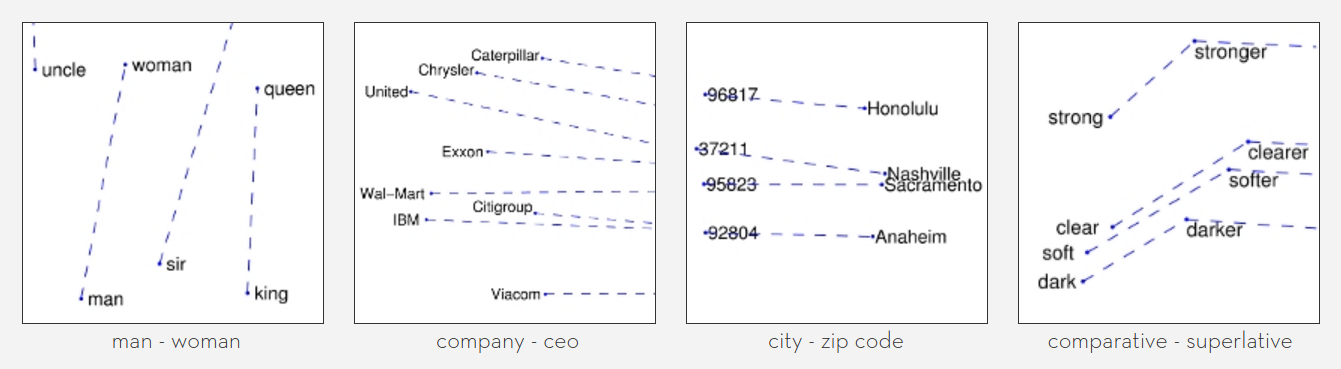
\includegraphics[scale=.225]{glove-space.png}
\flushright

\vspace{-.5cm}
\begin{tiny}
Pennington \emph{et al.}, https://nlp.stanford.edu/projects/glove/
\end{tiny}
\end{frame}


\begin{frame}

\[w_2 - w_1 \approx w_4 - w_3\]
\visible<2->{
\[w_4 \approx w_3 + w_2 - w_1\]
}

\vspace{.5cm}

\centering
\visible<3->{
\analogy{dog}{puppy}{cat}{?}
}

\begin{table}
\begin{tabular}{r l}
\centering
\visible<3->{
cat $+$ puppy $-$ dog }\visible<4->{ $\approx$ & kitten \\
& puppies \\
& pet \\
& beagle \\
& \hspace{.3cm} \vdots \\
& angiography \\
}
\end{tabular}
\end{table}
\end{frame}

\begin{frame}{Prior results}

Given the simplicity of the solving method, surprisingly high accuracy for some types of analogy questions.

\vspace{.3cm}
The most-used test set is probably the Google set (distributed with \texttt{word2vec}).
\begin{itemize}
\item Rather low diversity of categories---mostly geography and inflection
\item Results often reported on ``syntactic'' and ``semantic'' subsets; this division is too coarse to be useful
\end{itemize}

%\vspace{.3cm}
%No real attempts to explain differences in accuracy across categories.

\end{frame}

\begin{frame}{Word similarity}

High performance on many categories may be driven by \textbf{prior similarity} rather than successfully isolating components of meaning.
\vspace{.3cm}

Words in any relationship are usually fairly similar.

\visible<2->{
\vspace{.5cm}
\centering
\analogy{horse}{horses}{sailboat}{sailboats}

\vspace{.1cm}
horse $\approx$ horses, \\
sailboat $\approx$ sailboats
}

\visible<3->{
\vspace{.1cm}
hypothesis $=$ sailboat $+$ horses $-$ horse $\approx$ sailboat (!)
}

%\vspace{.1cm}
%$w_3 + w_2 - w_1 \approx w_3$


\end{frame}

\begin{frame}{Goal}
We designed a study that:
\begin{enumerate}
\item addresses a wide variety of categories, and
\item controls for prior similarity.
\end{enumerate}

\vspace{.5cm}
We want to \textbf{describe} and \textbf{explain} inter-category differences.
%\vspace{.5cm}
\end{frame}

\begin{frame}{Vectors}

\begin{itemize}
\item \texttt{word2vec}
\item Wikipedia
\item no case or punctuation
\item $d=200$, CBOW
\end{itemize}
\vspace{.5cm}

(Also experimented with GloVe, skip-gram, etc.)

\end{frame}

\begin{frame}{Test sets}

\visible<2->{
Microsoft Research (Mikolov \emph{et al.}, 2013a): inflectional relationships
\begin{itemize}
\item \analogy{cheap}{cheaper}{mighty}{mightier}
\item \analogy{learn}{learned}{think}{thought}
\item[] (etc.)
\end{itemize}
}

\vspace{.5cm}

\visible<3->{
Google (\texttt{word2vec}; Mikolov \emph{et al.}, 2013b): adds ``semantic'' categories
\begin{itemize}
\item \analogy{paris}{france}{havana}{cuba}
\item \analogy{austin}{texas}{minneapolis}{minnesota}
\item \analogy{king}{queen}{man}{woman}
\item[] (etc.)
\end{itemize}
}

\end{frame}

\begin{frame}{Test sets}
Better Analogy Test Set (BATS; Gladkova \emph{et al.}, 2016): \\
more derivational and semantic categories
\begin{itemize}
\item \analogy{helpful}{helpfulness}{righteous}{righteousness}
\item \analogy{bottle}{glass}{clothing}{fabric}
\item[] (etc.)
\end{itemize}
\vspace{.5cm}

\visible<2->{
SemEval 2012 (Jurgens \emph{et al.}, 2012): many, many more semantic categories
\begin{itemize}
\item \analogy{candy}{sweet}{snow}{cold}
\item \analogy{boy}{man}{gosling}{goose}
\item \analogy{bar}{drinking}{church}{worship}
\item[] (etc.)
\end{itemize}
}
\end{frame}

\begin{frame}{Test sets}

\begin{table}
\begin{tabular}{|r|c|c|}
\hline
\small{\textsc{Source}} & \small{\textsc{Categories}} & \small{\textsc{Analogies}} \\
\hline
\hline
Microsoft Research & 14 & 7,000 \\
Google (\texttt{word2vec}) & 14 & 19,544 \\
BATS & 40 & 95,625 \\
SemEval2012 & 79 & 30,082 \\
\hline
\textbf{Total} & 147 & 152,251 \\
\hline
\end{tabular}
\caption{\label{datasources} Summary of test data sources.}
\end{table}


\end{frame}

\begin{frame}{Metrics: Reciprocal rank}

Measure the \textbf{rank} of the correct answer in the entire vocabulary, ordered by similarity to hypothesis vector.
(Accuracy only measures if the correct answer is top-ranked.)
\vspace{.3cm}

\visible<2->{
Reciprocal of rank (RR) is more sensitive and forgiving than accuracy:

\begin{table}
\begin{tabular}{c|c|c}
rank & acc & RR \\
\hline
1 & 1 & 1 \\
2 & 0 & .5 \\
3 & 0 & .3333 \\
4 & 0 & .25 \\
\vdots & \vdots & \vdots \\
10526 & 0 & .0001 \\
\end{tabular}
\end{table}
}

\end{frame}
\begin{frame}{Metrics: Baseline}

\begin{itemize}
\item[] hypothesis vector $:=$ $w_2$ or $w_3$, whichever is better
\begin{itemize}
\item[] \emph{walk} :~\emph{walked} ::~\emph{\textbf{fly}} :~\emph{flew}
\item[] \emph{banana} :~\emph{\textbf{yellow}} ::~\emph{cherry} :~\emph{red}
\end{itemize}
\item ($w_3$ is better than $w_2$ in about 85\% of cases)
\end{itemize}


%\small
%(Baseline is useful for experiments but isn't a viable system design, as it has ``access'' to $w_4$.)
%\normalsize
\vspace{.3cm}

\visible<2->{
For each category of analogy questions, measure:
\begin{itemize}
\item mean RR using vector arithmetic hypothesis,
\item mean RR of the baseline hypothesis,
\item the difference between them.
\end{itemize}

%More solvable analogy questions $:=$ those that show a higher gain from baseline RR.
}
%Measure baseline reciprocal rank (BRR): the rank of $w_4$ using either $w_3$ or $w_2$ as the hypothesis vector.
%
%Report \textbf{RRG}: the reciprocal rank gain of the arithmetic strategy over baseline.

\end{frame}

\begin{frame}{Analogy supercategories}

We have 147 distinct categories of analogical relationships. \\
For visualization and analysis, consider supercategories:
\begin{itemize}
\item \textbf{inflection:} inflectional morphological relationships

(noun plural, adjective degree, verb tense)
\item \textbf{derivation:} derivational morphology (\emph{-tion}, \emph{un-})
\item \textbf{named entity semantics:} meanings of words with a single real-world referent (\emph{Vancouver, Beethoven})
\item \textbf{lexical semantics:} meanings of common nouns, adjectives, verbs, etc.
\end{itemize}

\end{frame}

\begin{frame}{Results: Inflection}
\centering
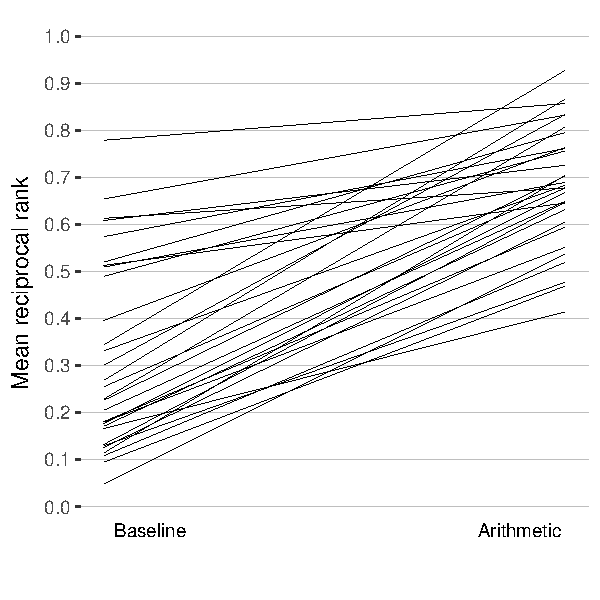
\includegraphics[scale=.8]{inflectional.pdf}
\end{frame}
\begin{frame}{Results: Inflection}
\centering
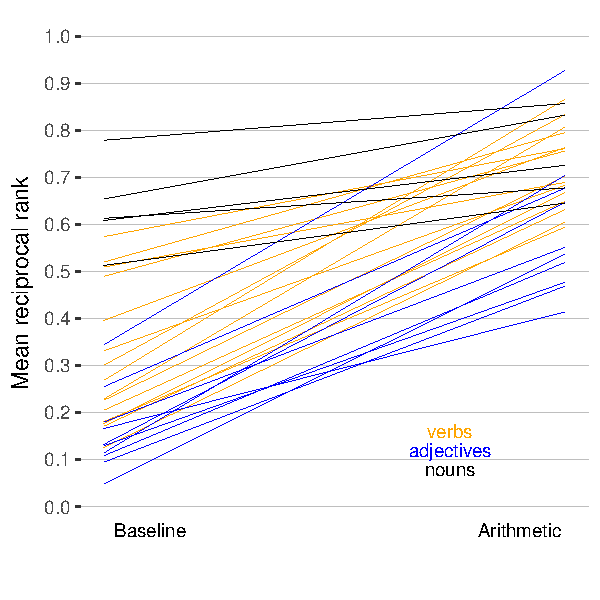
\includegraphics[scale=.8]{inflectional3.pdf}
\end{frame}

\begin{frame}{Results: Derivation}
\centering
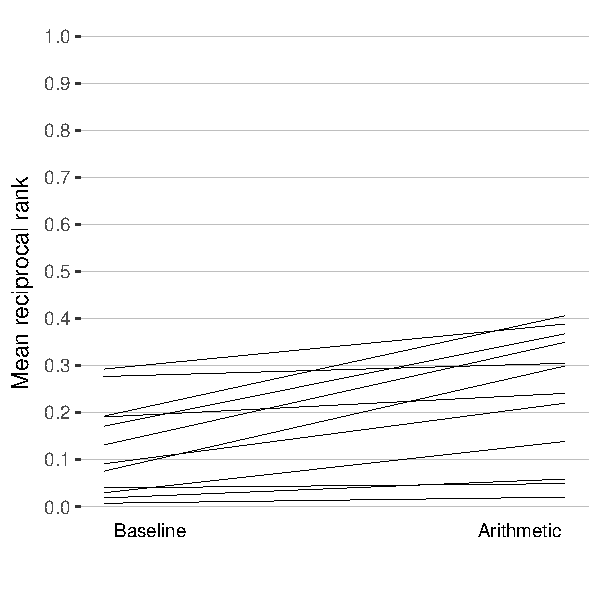
\includegraphics[scale=.8]{derivational.pdf}
\end{frame}
\begin{frame}{Results: Derivation}
\centering
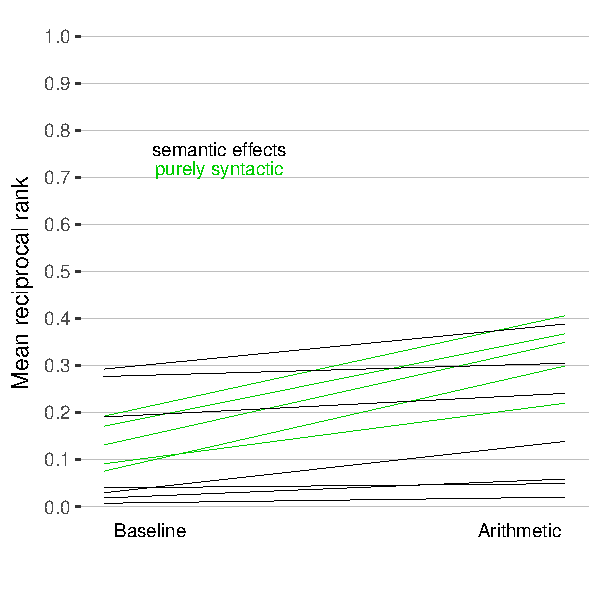
\includegraphics[scale=.8]{derivational2.pdf}
\end{frame}

\begin{frame}{Results: Named entities}
\centering
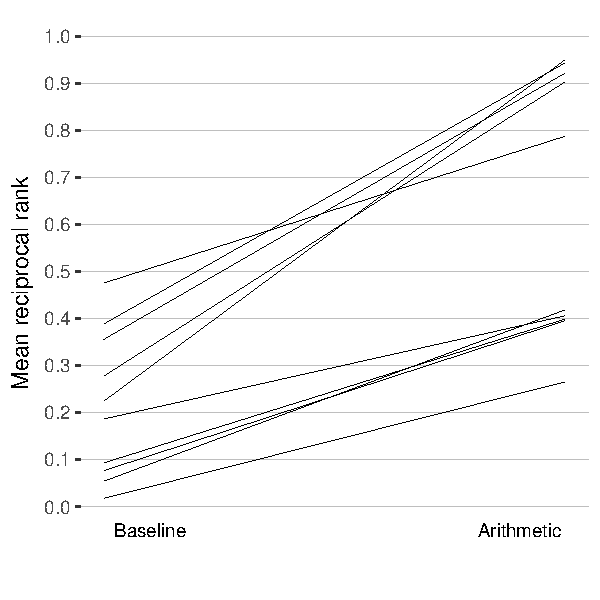
\includegraphics[scale=.8]{named.pdf}
\end{frame}
\begin{frame}{Results: Named entities}
\centering
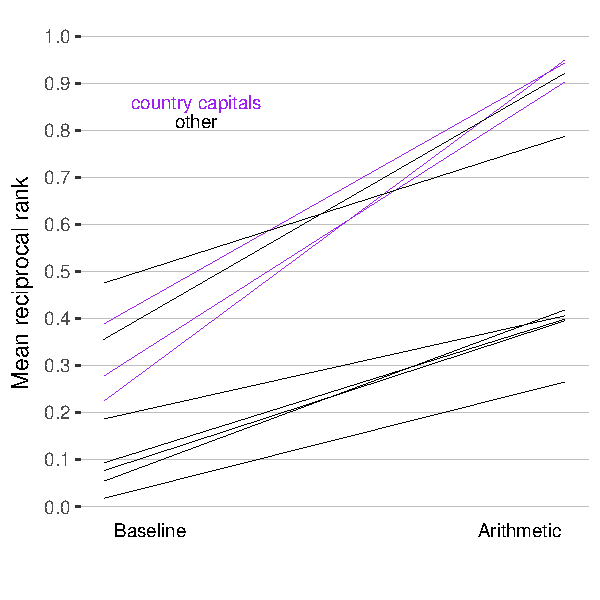
\includegraphics[scale=.8]{named2.pdf}
\end{frame}

\begin{frame}{Results: Lexical}
\centering
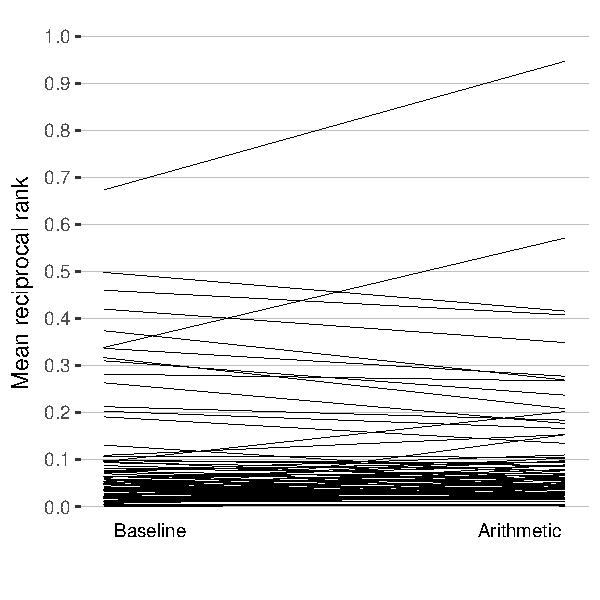
\includegraphics[scale=.8]{lexical.pdf}
\end{frame}
\begin{frame}{Results: Lexical}
\centering
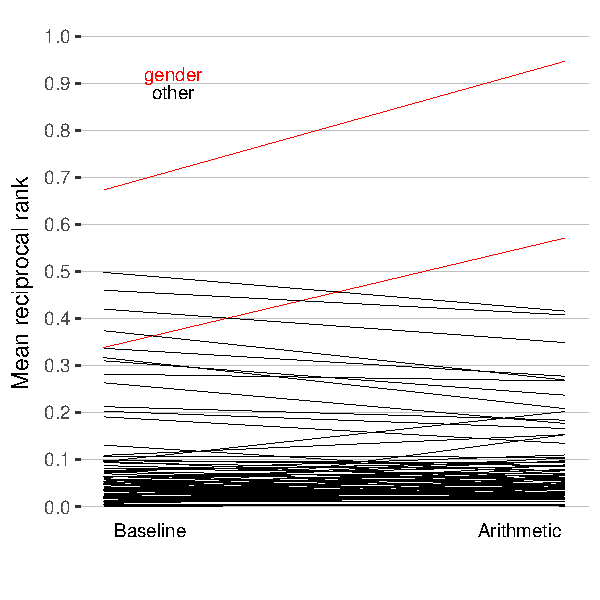
\includegraphics[scale=.8]{lexical2.pdf}
\end{frame}

\begin{frame}{Discussion: Derivation}

Linguists have proposed an inflection--derivation continuum. \\
Is performance worse with ``more derivational'' affixes?

\visible<2->{
\vspace{.3cm}
One hallmark of derivation is changing a word's syntactic class. \\
But for our results, a better continuum seems to be from morphemes with purely \textbf{syntactic} to purely \textbf{semantic} effects.
}

\visible<3->{
\begin{table}
\small
\begin{tabular}{c|c|c|c}
affix & syntactic? & semantic? & RR gain \\
\hline
-ment & V $\rightarrow$ N & minimal & .224 \\
-tion & V $\rightarrow$ N & minimal & .218 \\
-ly & A $\rightarrow$ Adv & minimal & .205 \\
-ness & A $\rightarrow$ N & minimal & .129 \\
-er & V $\rightarrow$ N & some? & .109 \\
un- & no (A) & yes & .062 \\
re- & no (V) & yes & .050 \\
-able & V $\rightarrow$ A & yes & .040 \\
-less & N $\rightarrow$ A & yes & .013 \\
-over & no (V) & yes & .009
\end{tabular}
\end{table}
}

\end{frame}

\begin{frame}{Discussion: Named entities}

Why the stark difference between named entities and other semantic relationships?
\vspace{.3cm}

Semantic theory supports differentiating common from named nouns. E.g., in Montagovian semantics:
\begin{itemize}
\item proper nouns denote \textbf{individuals} (type $e$)
\item common nouns denote \textbf{sets of individuals} (one-place predicates of type $\langle e,t\rangle$)
\end{itemize}
\vspace{.3cm}

\visible<2->{
Polysemy/ambiguity is a known problem for distributional approaches. If every \textbf{referent} is a sense, common nouns are extremely polysemous!
\vspace{.3cm}

Concretely: vector must \emph{simultaneously} model the word co-occurrences for every individual in the set.
}

\end{frame}

\begin{frame}{A unified account}

A relationship can be captured effectively by vector subtraction if it has \textbf{predictable distributional consequences}.
\vspace{.3cm}

\visible<2->{
Sets of co-occurrence differences between terms in a pair should be \textbf{regular} and \textbf{small}.
\vspace{.3cm}
}

%The set of co-occurrences unique to one word or the other in a pair should be \textbf{small} and \textbf{regular}.

\visible<3->{
\begin{itemize}
\item Inflection has predictable effects with agreement and syntax.
Adjectives especially:

\begin{itemize}
\item[] \emph{that is \textcolor{orange}{a} \textbf{cheap} tuxedo}
\item[] \emph{that is \textcolor{orange}{a} \textbf{cheaper} tuxedo \textcolor{orange}{than} \ldots}
\item[] \emph{that is \textcolor{orange}{the} \textbf{cheapest} tuxedo}
\end{itemize}
}

\visible<4->{
\dots and verbs too:

\begin{itemize}
\item[] \emph{she \textbf{ran} out of time}
\item[] \emph{she \textcolor{orange}{is} \textbf{running} out of time}
\item[] \emph{she \textcolor{orange}{has} \textbf{run} out of time}
\end{itemize}
}


\end{itemize}

\end{frame}
\begin{frame}{A unified account}

\begin{itemize}
\item Derivation is less regular than inflection. More importantly, its distributional effects are less automatic and predictable:

\begin{itemize}
\item[] \emph{Billy was a \textbf{slow} \textcolor{orange}{runner}}
\item[] \emph{Billy \textcolor{orange}{ran} \textbf{slowly}}
\item[] \hspace{1.5cm}vs.
\item[] \emph{their \textcolor{orange}{investments} have been very \textbf{prudent} this year}
\item[] \emph{they \textcolor{orange}{invested} very \textbf{prudently} this year}
\end{itemize}

\item Adverbs tend to co-occur with verbs and adjectives with nouns, but these words do not belong to \textbf{closed classes} as they tend to with inflection.

\end{itemize}
\end{frame}
\begin{frame}{A unified account}

What about semantics?

\begin{itemize}
\item Less polysemous nouns will have ``tighter'' distributions: lower diversity of co-occurrences, thus smaller sets of differences.
Named entities are especially non-polysemous.
\begin{itemize}
\item
The relationship between every \emph{dog} and every \emph{puppy} is less consistent than the relationship between every \emph{Netherlands} and every \emph{Amsterdam}.
\end{itemize}

\visible<2->{
\item Gendered nouns agree with pronouns---a closed class, as seen with inflectional relationships.

\begin{itemize}
\item[] \emph{when the \textbf{boy} dropped \textcolor{orange}{his} ice cream, \textcolor{orange}{he} cried}
\item[] \emph{when the \textbf{girl} dropped \textcolor{orange}{her} ice cream, \textcolor{orange}{she} cried}
\end{itemize}
}

\end{itemize}

\end{frame}

\begin{frame}{Conclusion}

We have arrived at an explanation grounded in linguistic and distributional theory that accounts for the effects observed.
\begin{itemize}
\item Should work further to verify the claim that certain distributional differences are more regular (although the analogy task \emph{does} measure that directly).
\end{itemize}

\vspace{.3cm}
Recommend: Test a wide variety of questions. Use a baseline. Don't rely on coarse splits like ``syntactic/semantic.''

%\vspace{.3cm}
%Contact: gregpfinley@gmail.com

\vspace{.4cm}
\hrule
\vspace{.4cm}
\small
All code, results, and figures will be available at: https://github.com/gpfinley/analogies

\vspace{.3cm}
This work was partially supported by the National Institute of General Medical Sciences (GM102282).

\end{frame}
%\begin{frame}{Complications}
%...lots of complications to talk about and be aware of (borrow from paper); i think it's important to bring them up at a conference since it's all about meeting people and hashing out ideas
%\end{frame}

%\begin{frame}{Recommendations}
%
%When reporting analogy results:
%\begin{itemize}
%\item Don't use the ``syntactic''/``semantic'' Google set split!
%\end{itemize}
%
%...don't use the syntactic/semantic split for the Google set
%
%Don't assume that vector difference can capture purely semantic relationships. That seems to be the exception rather than the rule.
%\end{frame}
%
%\begin{frame}{Future work}
%
%Quantitatively verify the assertion that distributions are more regular for certain relationships.
%
%Investigate the observed hierarchy 
%
%...
%
%
%Further experiments with 
%
%\end{frame}




% Uncomment these lines for an automatically generated outline.
%\begin{frame}{Outline}
%  \tableofcontents
%\end{frame}

\end{document}
